% "{'classe':('PSI'),'chapitre':'stat_mam','type':('application'),'titre':'Modélisation des actions mécaniques', 'source':'Stéphane Genouël','comp':('B2-14','C1-05','C2-07'),'corrige':True}"
%\setchapterimage{fig_00.jpg}
\chapter*{Application \arabic{cptApplication} \\ 
Modélisation des actions mécaniques -- \ifprof Corrigé \else Sujet \fi}
\addcontentsline{toc}{section}{Application \arabic{cptApplication} : Modélisation des actions mécaniques  -- \ifprof Corrigé \else Sujet \fi}

\iflivret \stepcounter{cptApplication} \else
\ifprof  \stepcounter{cptApplication} \else \fi
\fi

\setcounter{question}{0}
\marginnote{Ressources de Stéphane \textsc{Genouël}.}
\marginnote[1cm]{
\UPSTIcompetence[2]{B2-14}
\UPSTIcompetence[2]{C1-05}
\UPSTIcompetence[2]{C2-07}
}



\subsection*{Exercice 1 : Assemblage par frettage}

Le frettage consiste à encastrer deux pièces en utilisant le phénomène d’adhérence. 
 
Avant l’assemblage réalisé à l’aide d’une presse, l’arbre 1 
possède un diamètre légèrement supérieur à celui de l’alésage 
(trou cylindrique) de la pièce 2 dans laquelle il vient se loger. 
 
Après frettage, il subsiste donc une pression de contact $p$ 
(souvent supposée uniforme sur toute la surface de contact) 
entre les deux pièces. 


\begin{marginfigure}
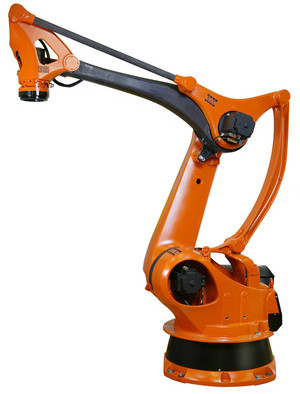
\includegraphics[width=\linewidth]{fig_01}
\end{marginfigure}
 
Les caractéristiques de cet assemblage par frettage sont les suivantes : 
\begin{itemize}
\item $R$ : rayon de l’arbre 1;
\item $L$ : longueur du contact; 
\item $f$ : facteur d’adhérence entre les deux pièces.
\end{itemize}





\begin{obj}
Déterminer l’effort axial maximal transmissible et le couple maximal transmissible d’une pièce à 
l’autre.
\end{obj}

\subsection*{Effort axial maximal transmissible}


L’effort axial maximal transmissible correspond à la valeur maximale de la 
composante axiale de la résultante de l’action mécanique qui peut être transmise 
d’une pièce à l’autre sans qu’elles se désolidarisent. 
 
Pour simplifier notre étude, on considère la pièce 2 fixe et on cherche à déterminer 
la composante axiale de la résultante de l’action mécanique à appliquer à la pièce 1 
pour atteindre le glissement de 1/2 suivant $-\vect{z}$. 


\begin{marginfigure}
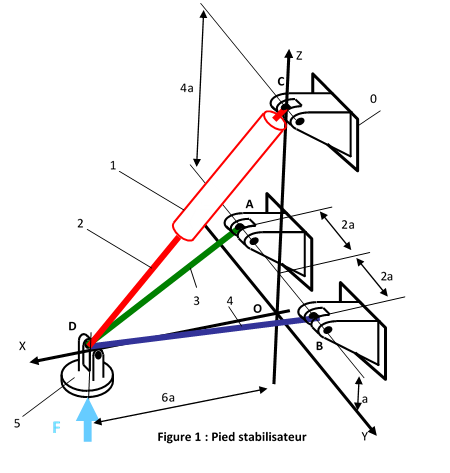
\includegraphics[width=.8\linewidth]{fig_02}
\end{marginfigure}


\question{Refaire en grand les 2 schémas : un 
dans le plan $(\vect{y}, \vect{z})$ et l’autre dans le plan $(\vect{x}, \vect{y})$, 
en plaçant les actions élémentaires normale et 
tangentielle de 2 sur 1 en un point $Q$ 
quelconque de la surface de contact. }

\begin{marginfigure}
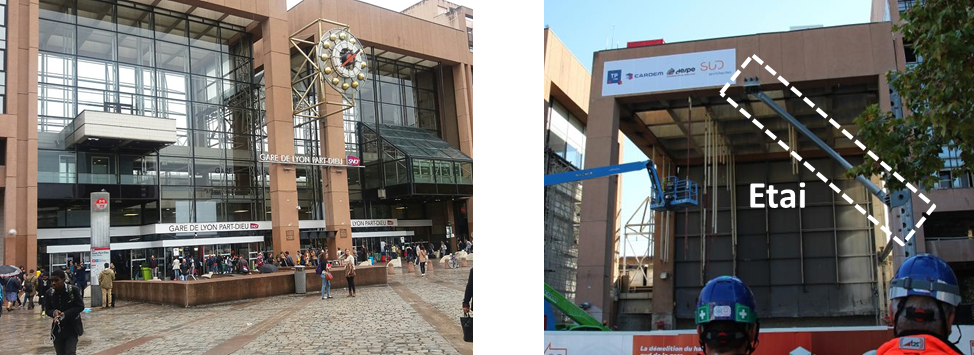
\includegraphics[width=.8\linewidth]{fig_03}
\end{marginfigure}


\question{Exprimer $\vect{dF_{2\rightarrow 1}(Q)}$.}

\question{Déterminer la résultante axiale maximale transmissible en fonction de $p$ et des 
caractéristiques géométriques du frettage. }

\ifprof
\begin{corrige}
Exprimons le torseur des actions mécaniques sous sa forme locale en un point $M$ : 

$$
\torseurl{d\vectf{2}{1}}{d\vectm{M}{2}{1}=\vect{0}}{M}
$$

La forme globale au point O est alors donnée par :

$$
\torseurstat{T}{2}{1} = \torseurl{\vectf{2}{1} = \int d\vectf{2}{1}}{\vectm{M}{2}{1} = \int d\vectm{M}{2}{1}= \int \vect{OM}\wedge d\vectf{2}{1}}{M}
$$




\textbf{Calculons $\vectf{2}{1}$.}

$$
\vectf{2}{1} = \int d\vectf{2}{1} = \iint p \vect{-r} dS = -p \iint  \vect{r} dS
= -p \iint  \left(\cos\theta\vect{x}+\sin\theta\vect{y} \right) dS $$

$$
\vectf{2}{1}
= -p \int\limits_{-L/2}^{L/2} \int\limits_{-\pi/2}^{\pi/2}   \left(\cos\theta\vect{x}+\sin\theta\vect{y} \right) Rd\theta dz
= -p R L \int\limits_{-\pi/2}^{\pi/2}   \left(\cos\theta\vect{x}+\sin\theta\vect{y} \right) d\theta 
$$
$$
\vectf{2}{1}
= -p R L \left(\int\limits_{-\pi/2}^{\pi/2}   \cos\theta\vect{x}d\theta + \int\limits_{-\pi/2}^{\pi/2} \sin\theta\vect{y} d\theta \right)
= -p R L \left(\left[\sin\theta \right]_{-\pi/2}^{\pi/2}\vect{x}
+\left[ -\cos\theta\right]_{-\pi/2}^{\pi/2}\vect{y}
\right)
$$

$$
\vectf{2}{1}
= -p R L \left(2\vect{x}
+0\vect{y}
\right) = -2pRL\vect{x}
$$

$2RL$ est appelée surface projetée du cylindre. Elle correspond au produit du diamètre par sa longueur.

\vspace{.5cm}

\textbf{Calculons $\vectm{M}{2}{1}$.}
$$
\vectm{M}{2}{1} = \int d\vectm{M}{2}{1}= \int \vect{OM}\wedge d\vectf{2}{1}
$$

$$
\vectm{M}{2}{1} = -p \iint R\vect{r} \wedge \vect{r}dS = \vect{0}
$$

Au final, 
$$
\torseurstat{T}{2}{1} = \torseurl{\vectf{2}{1} = -2pRL\vect{x}}{\vectm{M}{2}{1} =  \vect{0}}{M}
$$

\end{corrige}
\else
\fi





%
%\subparagraph{}
%\textit{Calculer $\vectf{2}{1}$ lorsque la pression est de la forme : $p(\theta)=p_0\cos\theta$ pour $\theta\in[-\pi/2,\pi/2]$.}
\ifprof
\begin{corrige}

Dans ce cas : 
$$
\vectf{2}{1} = \int d\vectf{2}{1} = \iint p(\theta) \vect{-r} dS 
= - p_0R\iint\cos\theta  \left(\cos\theta\vect{x}+\sin\theta\vect{y} \right)  d\theta dz$$

$$
\vectf{2}{1} 
= - p_0 L R\int\limits_{-\pi/2}^{\pi/2}\cos\theta  \left(\cos\theta\vect{x}+\sin\theta\vect{y} \right)  d\theta$$

$$
\int\limits_{-\pi/2}^{\pi/2}\cos^2\theta  d\theta = \dfrac{\pi}{2}
\quad 
\text{et}
\quad
\int\limits_{-\pi/2}^{\pi/2}\cos\theta \sin\theta  d\theta = 0
$$
Au final :
$$
\vectf{2}{1} 
= - p_0 L R \dfrac{\pi}{2}\vect{x}$$
\end{corrige}
\else
\fi




\subsection*{Couple maximal transmissible}


Le couple (ou moment) maximal transmissible correspond à la valeur maximale 
de la composante sur l’axe $\vect{z}$ du moment résultant de l’action mécanique qui peut 
être transmise d’une pièce à l’autre sans qu’elles se désolidarisent. 
 
Pour simplifier notre étude, on considère la pièce 2 fixe et on cherche à 
déterminer la composante sur l’axe $\vect{z}$ du moment résultant de l’action mécanique 
à appliquer à la pièce 1 pour atteindre le glissement de 1/2 autour de $\vect{z}$.
 

\begin{marginfigure}
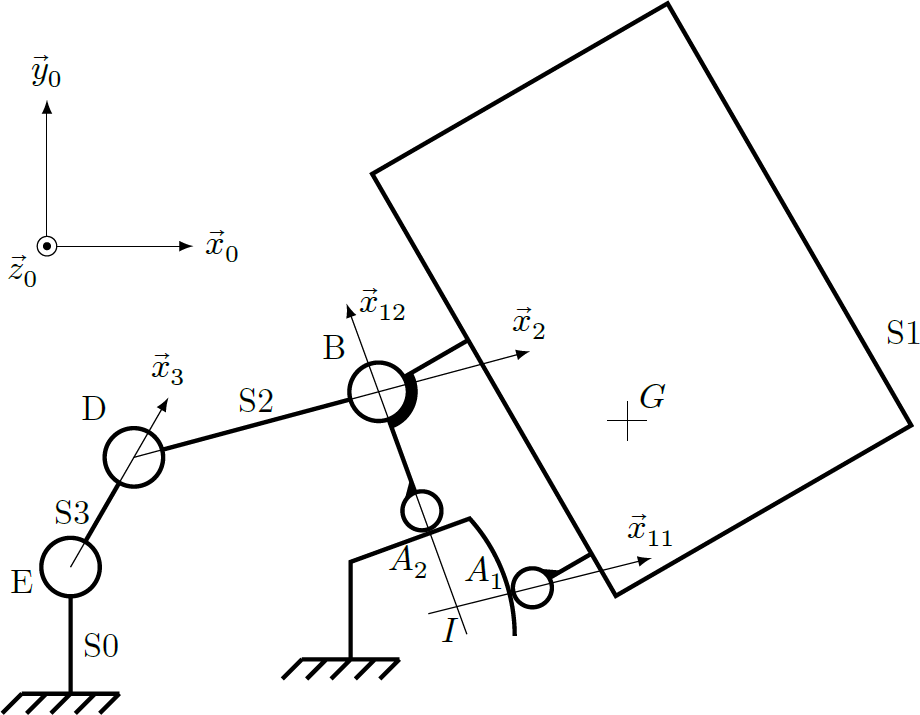
\includegraphics[width=.8\linewidth]{fig_04}
\end{marginfigure}



\question{Refaire en grand les 2 schémas  : un 
dans le plan $(\vect{y}, \vect{z})$ et l’autre dans le plan $(\vect{x}, \vect{y})$, 
en plaçant les actions élémentaires normale et 
tangentielle de 2 sur 1 en un point $Q$ 
quelconque de la surface de contact. }


\begin{marginfigure}
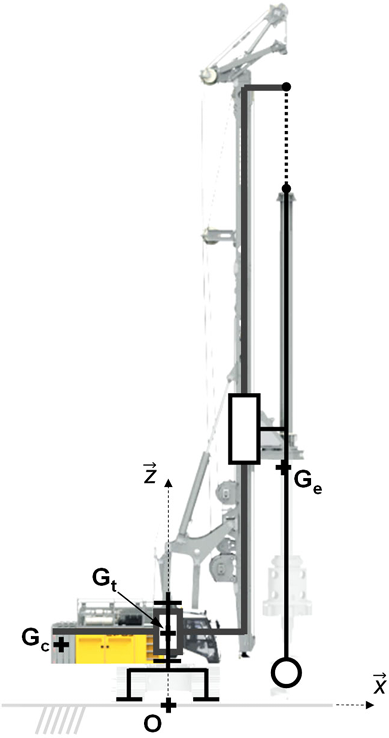
\includegraphics[width=.8\linewidth]{fig_05}
\end{marginfigure}



\question{Exprimer $\vect{dF_{2\rightarrow 1}(Q)}$.}

\question{Déterminer le couple maximal transmissible en fonction de $p$ et des 
caractéristiques géométriques du frettage.}


\subsection*{Exercice 2 : Embrayage à friction mono disque de véhicules automobiles (surfaces de friction plane)}

Situé en amont des boîtes à vitesses, l'embrayage mono disque a pour rôle de désolidariser le moteur de la 
boîte afin de pouvoir changer de rapports, ou lorsque le véhicule est arrêté moteur tournant au ralenti. 

\begin{marginfigure}
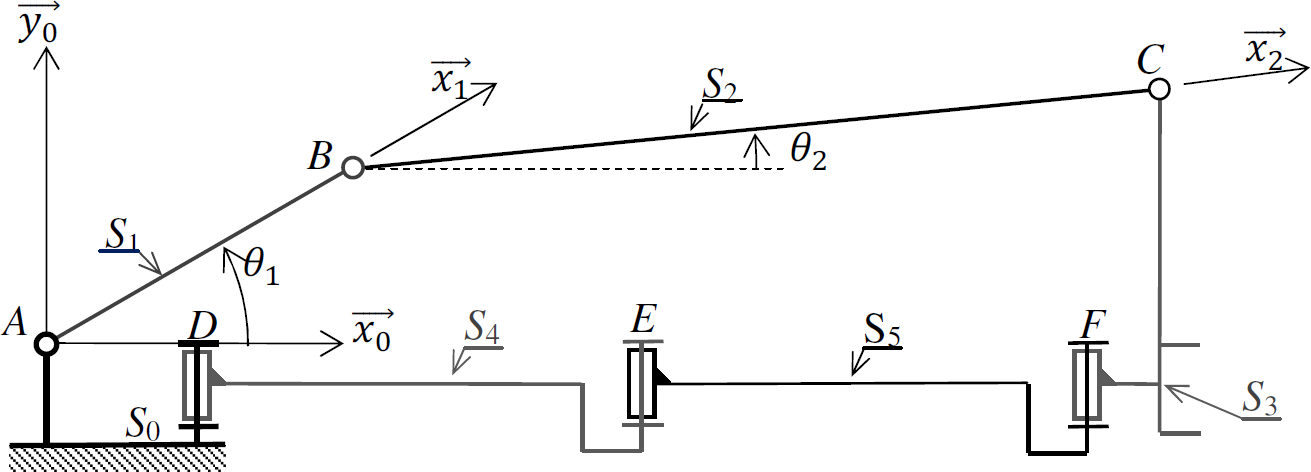
\includegraphics[width=\linewidth]{fig_06}
\end{marginfigure}

\textbf{Position embrayée :} le disque est fortement serré entre deux surfaces lisses (plateau et volant) par la 
pression des ressorts. Le tout tournera donc d'un bloc, sans glissement et sans pertes. 

\textbf{Position débrayée :} la poussée du conducteur sur la pédale contrebalance la force des ressorts. Le disque, sous l'effet des vibrations, coulisse alors légèrement sur ses cannelures pour se positionner entre les surfaces lisses (plateau et volant), sans les toucher. Les vitesses angulaires du volant-plateau (solidaires du vilebrequin) et du disque (solidaire des roues par l'intermédiaire de la transmission) peuvent alors différer 
sans que le disque ne frotte. 


On modélise l'embrayage par 2 disques creux identiques (1 et 2) en contact grâce à une 
action axiale $\vect{F_a}$. 
 
Le rayon intérieur des 2 disques vaut : $R_{\text{min}}$. 
Le rayon extérieur des 2 disques vaut : $R_{\text{max}}$. 
On donne $f$ le facteur d’adhérence entre les deux pièces. 



\begin{marginfigure}
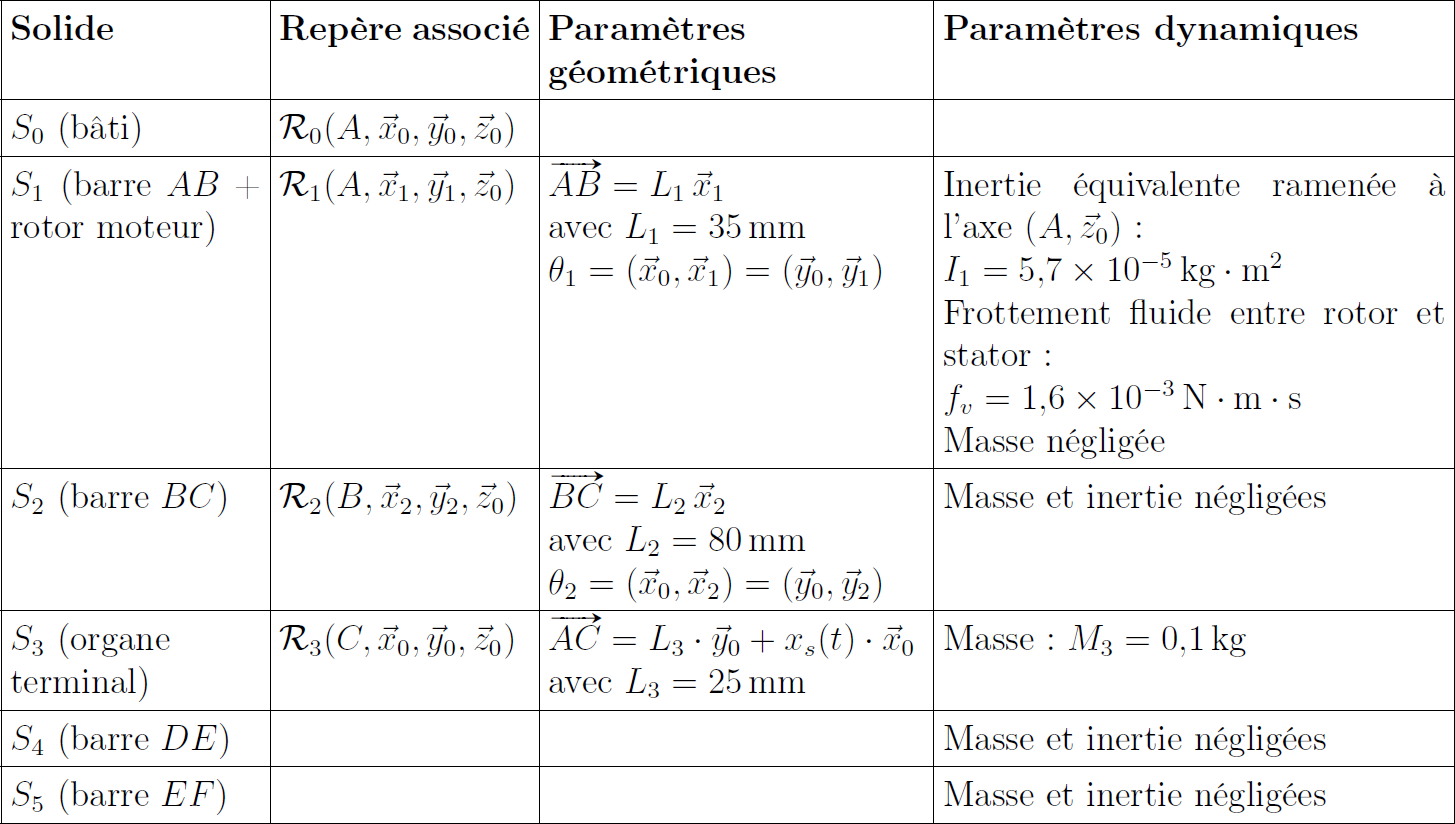
\includegraphics[width=\linewidth]{fig_07}
\end{marginfigure}

\question{Refaire en grand les 2 schémas ci-dessus : un dans le plan $(\vect{y}, \vect{z})$ et l’autre dans le plan $(\vect{x}, \vect{y})$, en plaçant les actions élémentaires normale et tangentielle de 2 sur 1 en un point $Q$ quelconque de la surface de contact.}

\question{Exprimer $\vect{dF_{2\rightarrow 1}(Q)}$.}

\question{Déterminer le couple maximal transmissible en fonction de $p$ et des caractéristiques 
géométriques de l’embrayage.}

\question{Déterminer l’action axiale $\vect{F_a}$ qui crée les $\vect{\text{d}N}$ en fonction de $p$ et des caractéristiques géométriques de l’embrayage.}

\question{En déduire le couple maximal transmissible en fonction de $F_a$ (et non en fonction de $p$) et des caractéristiques géométriques de l’embrayage.}

\ifprof

\begin{corrige}

\textbf{Expression du couple infinitésimal}
$$
d\vectm{\text{Plateau}}{\text{Disque}}{O} =
d\vectm{P}{D}{O} =  \vect{OM}\wedge d\vectf{P}{D}
$$

\textbf{Expression de la résultante infinitésimale}

$$
d\vectf{P}{D} = d\vect{N(P\rightarrow D)}+d\vect{T(P\rightarrow D)}
$$

\textbf{Expression de l'effort normal}

$$
d\vect{N(P\rightarrow D)} = p \vect{n} d\mathcal{S} = -p \vect{z} d\mathcal{S}
$$

\textbf{Expression de l'unité de surface}

$$
d\mathcal{S} = \rho d\theta d\rho
$$

\textbf{Expression de l'effort tangentiel}

D'après le modèle de Coulomb, on commence par identifier le vecteur $\vectv{M}{D}{P}$.
Le vecteur tangentiel est donc opposé à ce dernier. A la limite du glissement on a alors : 
$$
d\vect{T(P\rightarrow D)} = -f ||d\vect{N(P\rightarrow D)}|| \vect{v}    = fp d\mathcal{S}\vect{v}
$$

\textbf{Calcul final}

On note $\vect{OM}=\rho\vect{u}$ :

\begin{eqnarray*}
\vectm{O}{P}{D}  
&=& d\vectm{O}{P}{D}  \\
&=& \int \vect{OM}\wedge d\vectf{P}{D} \\
&=& \int \rho\vect{u} \wedge \left( d\vect{N(P\rightarrow D)}+d\vect{T(P\rightarrow D)} \right)\\
&=& \int \rho\vect{u} \wedge \left( -p \vect{z} d\mathcal{S} +fp d\mathcal{S}\vect{v} \right)\\
&=& \iint p\rho\vect{v} d\mathcal{S} +\iint pf\rho  \vect{z}d\mathcal{S} = 
\iint p\rho\vect{v} \rho d\theta d\rho +\iint pf\rho  \vect{z}\rho d\theta d\rho \\
\end{eqnarray*}

\begin{eqnarray*}
\iint p\rho\vect{v} \rho d\theta d\rho = \iint p\rho\left(\cos\theta\vect{y}-\sin\theta\vect{x} \right) \rho d\theta d\rho \\
=\iint p\rho\cos\theta\vect{y}  \rho d\theta d\rho-\iint p\rho \sin\theta\vect{x}  \rho d\theta d\rho \\
=p \vect{y}  \int\limits_{r}^{R} \int\limits_{0}^{2\pi}\cos\theta d\theta \rho^2 d\rho- p\vect{x}\int\limits_{r}^{R} \int\limits_{0}^{2\pi} \sin\theta  \rho^2 d\theta d\rho \\
=p \left[ \sin\theta\right]_{0}^{2\pi}\left[ \dfrac{1}{3}\rho^3\right]_{r}^{R}\vect{y}\
 -
p \left[ -\cos\theta\right]_{0}^{2\pi}\left[ \dfrac{1}{3}\rho^3\right]_{r}^{R}\vect{x} = \vect{0}
\end{eqnarray*}

\begin{eqnarray*}
\iint pf\rho^2 \vect{z} d\theta d\rho =
pf \left[ \theta\right]_{0}^{2\pi}\left[ \dfrac{1}{3}\rho^3\right]_{r}^{R} \vect{z}\\
= pf2\pi \dfrac{R^3-r^3}{3} 
\end{eqnarray*} 

Enfin, en notant $F_r$ l'effort (uniformément réparti) exercé par le ressort sur toute la couronne, on a donc :
$$
p=\dfrac{F_r}{\pi \left(R^2-r^2 \right)}
$$

Au final : 

$$ \vectm{O}{P}{D}  
= f\dfrac{2}{3} \dfrac{R^3-r^3}{R^2-r^2} F_r
$$
\end{corrige}

\else
\fi


\subsection*{Exercice 3 : Embrayage conique des synchroniseurs de boite de vitesses (surface de friction coniques)} 

\begin{marginfigure}
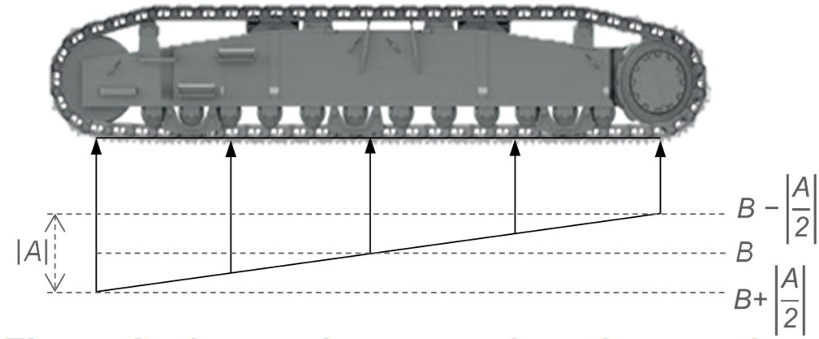
\includegraphics[width=\linewidth]{fig_08}
\end{marginfigure}

Les boîtes de vitesses automobiles ont pour particularité d'avoir tous leurs engrenages en prise. 
Les pignons et roues situés sur l’arbre primaire (arbre qui sera lié à l'arbre moteur) sont en liaison pivot sur ce dernier donc ils tournent tous à des vitesses différentes autour de cet arbre. Ces pignons et roues sont 
appelés pignons « fous » et roues « folles » 

Les pignons et roues situés sur l’arbre secondaire sont solidaires de ce dernier donc ils tournent tous à la même vitesse. 

Le rôle de la boîte de vitesses est de mettre en liaison encastrement un des pignons (ou roues) fous de l’arbre primaire avec l’arbre primaire. Or pour pouvoir solidariser un des pignons fous et son arbre, il faut synchroniser leurs régimes de vitesses, et c'est là le rôle des synchroniseurs. 


On modélise le pignon fou et l'anneau de synchronisation par 2 cônes en contact 
grâce à une action axiale $\vect{F_a}$. 
 
Le rayon maximal des 2 cônes vaut : $R_{\text{max}}$. 
Le rayon minimal des 2 cônes vaut : $R_{\text{min}}$. 
Le demi-angle au sommet des 2 cônes vaut $\alpha$. 
On donne $f$le facteur d’adhérence 
entre les deux pièces.



\begin{marginfigure}
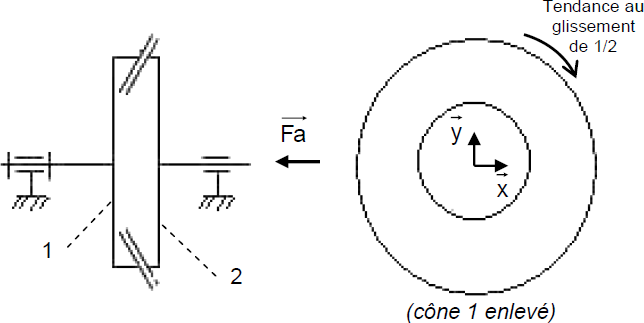
\includegraphics[width=\linewidth]{fig_09}
\end{marginfigure}


\question{Refaire en grand les 2 schémas ci-dessus : un dans le plan $(\vect{y}, \vect{z})$ et l’autre dans le plan $(\vect{x}, \vect{y})$, en plaçant les actions élémentaires normale et tangentielle de 2 sur 1 en un point $Q$ quelconque de la surface de contact.}

\question{Exprimer $\vect{dF_{2\rightarrow 1}(Q)}$.}

\question{Déterminer le couple maximal transmissible en fonction de $p$ et des caractéristiques 
géométriques de l’embrayage.}

\question{Déterminer l’action axiale $\vect{F_a}$ qui crée les $\vect{dN}$ en fonction de $p$ et des caractéristiques géométriques de l’embrayage.}

\question{En déduire le couple maximal transmissible en fonction de $F_a$ (et non en fonction de $p$) et des caractéristiques géométriques de l’embrayage.}


%\newpage
%
%
%\subsection*{Modélisation des actions mécaniques de contact sur un palier lisse}
%
%
%On souhaite déterminer le modèle global des actions mécaniques de contact sur un palier lisse, composant technologique pour le guidage en rotation.
%
%On donne le modèle local :
%\begin{itemize}
%\item les surfaces de contact sont limitées par un demi cylindre de longueur $L$ et de rayon $R$;
%\end{itemize}
%
%\textbf{On considère dans un premier temps que la répartition de pression est uniforme.}
%
%La pression $p$ est uniforme sur chaque élément $dS$ situé autour du point $M$.
%
%
%\begin{center}
%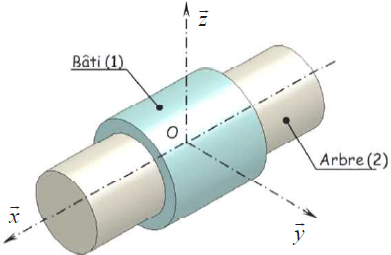
\includegraphics[width=.9\linewidth]{png/fig5}
%\end{center}
%
%
%
%\begin{center}
%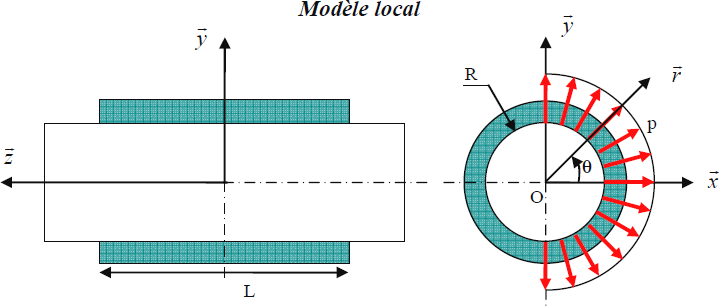
\includegraphics[width=\linewidth]{png/fig6}
%\end{center}

%\setcounter{exo}{0}
\question{Déterminer le modèle global de l'action mécanique de l'arbre 2 sur le bâti 1 sous forme d'un torseur exprimé au point $O$.}

\subsection*{Couple transmis par une clavette}
%\setcounter{exo}{0}


\begin{marginfigure}
\begin{center}
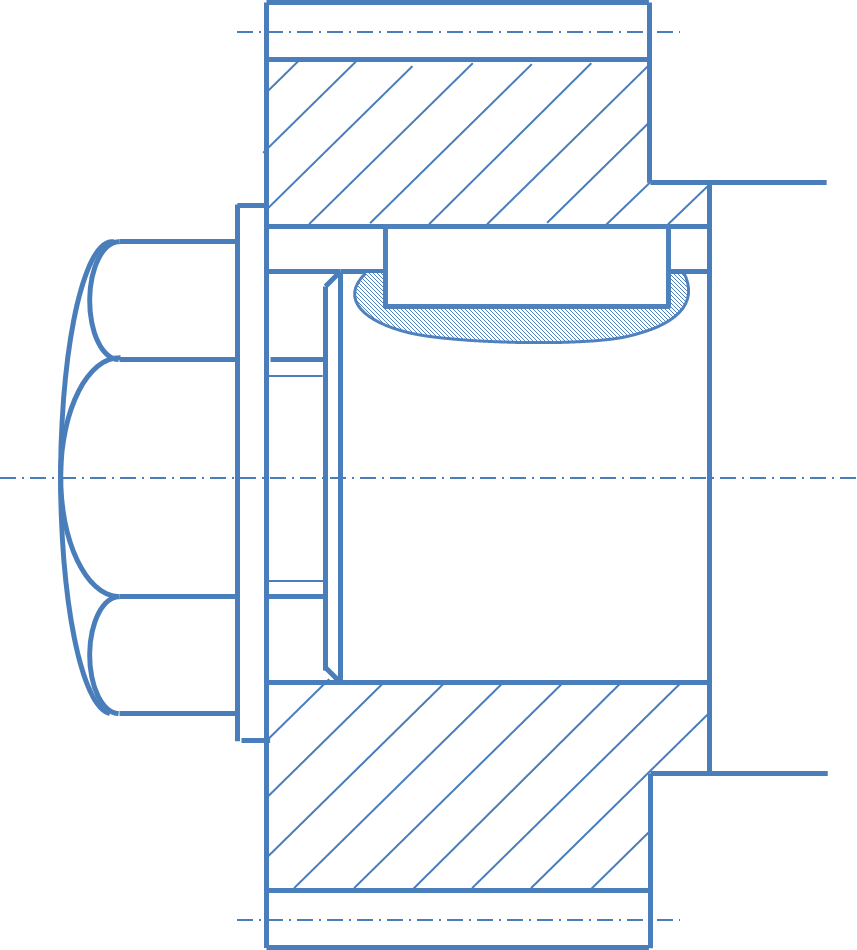
\includegraphics[width=.7\linewidth]{clavette}
\end{center}

\end{marginfigure}
On cherche à connaître le couple transmissible autour de $\vect{z}$, axe du pignon.

La clavette est de hauteur $2h$ et de largeur $l$. On note $p$ le champ de pression uniforme du pignon sur une demi-clavette. $p$ est appelée pression de matage. 

$O$ est un point de l'axe.


\question{Déterminer le couple transmissible par la clavette.}

\ifprof
(A revoir, notamment les bornes d'intégrations sur la hauteur de la clavette).


$$
\vectm{O}{\text{Pignon}}{\text{Arbre}} \cdot \vect{z} = 
\vectm{O}{P}{A} \cdot \vect{z} 
= \int \vect{OM}\wedge d\vectf{P}{A} \cdot \vect{z}
= \int x\vect{x} \wedge p \vect{y}  dx dz \cdot \vect{z}
$$

$$
\vectm{O}{\text{Pignon}}{\text{Arbre}} \cdot \vect{z} 
= \int\limits_{0}^{l}\int\limits_{R-h/2}^{R+h/2} px\underbrace{\left( \vect{x} \wedge  \vect{y}\right)\cdot \vect{z}}_1  dx dz 
= pl\int\limits_{R-h/2}^{R+h/2} x  dx =\dfrac{1}{2}pl\left(\left(R+h/2 \right)^2-\left( R-h/2\right)^2 \right)
$$


$$
\vectm{O}{\text{Pignon}}{\text{Arbre}} \cdot \vect{z} 
=hplR
$$

Ce résultat peut paraître logique : la force exercée sur la clavette s'exprime par $phl$. Le bras de levier du glisseur correspond au rayon de l'arbre auquel on ajoute un quart de hauteur de clavette.


Attention, si on considère que le couple est transmis par l'ensemble du flanc de la clavette, le moment transmissible est de la forme : 

$$
\vectm{O}{\text{Pignon}}{\text{Arbre}} \cdot \vect{z} 
=hLpR
$$
\else
\fi

\ifprof
\else
\begin{marginfigure}
\centering

\includegraphics[width=3cm]{Cy_11_Ch_01_02_qr}
\end{marginfigure}
\fi